
\chapter{Problem Statement}
\graphicspath{{Chapter_3/Vector/}{Chapter_3/}}

In this section, we investigate the application of compositional runtime enforcement in underwater robotic swarms and compare its effectiveness against the conventional monolithic approach. The focus is on enhancing a Multi-Robot Coverage Path Planning (MRCPP) algorithm tailored for mapping underwater vegetation, particularly within seagrass beds. This study evaluates how these runtime enforcement strategies influence key aspects of the MRCPP algorithm, such as performance, scalability, and adaptability, when operating in dynamic and unpredictable underwater environments. Through this comparison, we aim to identify a more efficient and robust framework for ensuring mission success in such challenging scenarios.

\section{DARP: Divide Areas Algorithm for Optimal Multi-Robot Coverage Path Planning}
\rhead{DARP}
\label{DARP}

In this paper, we will be using the algorithm discussed in \cite{kapoutsisdarp}.

In essence, the DARP algorithm follows a cyclic coordinate descent optimization scheme updating each robot’s territory separately but towards achieving the overall multi-robot Coverage Path Planning (mCPP) objectives. After the desired area division is achieved, we use the Spanning Tree Coverage (STC) algorithm to produce the optimal path for each robot, in order to achieve full coverage of the area of interest. This algorithm is able to account for prior-defined obstacles too.

\begin{figure*}[!ht]
	\centering
	% First row of subfigures
	\subfloat[Initial cells discretization, robots' cell, and obstacles \label{fig:darp1}]{
		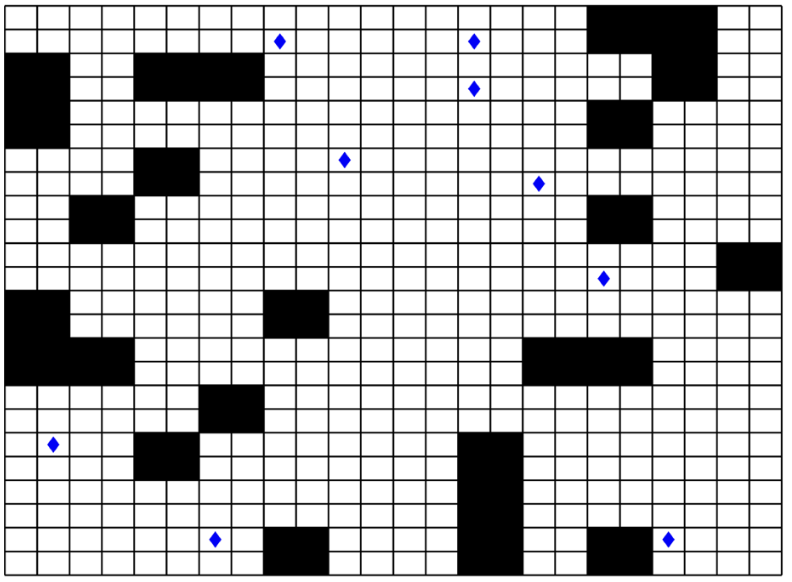
\includegraphics[width=0.45\columnwidth]{fig/darp1.png}
	}
	\hspace{0.1em}
	\subfloat[DARP outcome - robots’ exclusive areas \label{fig:darp2}]{
		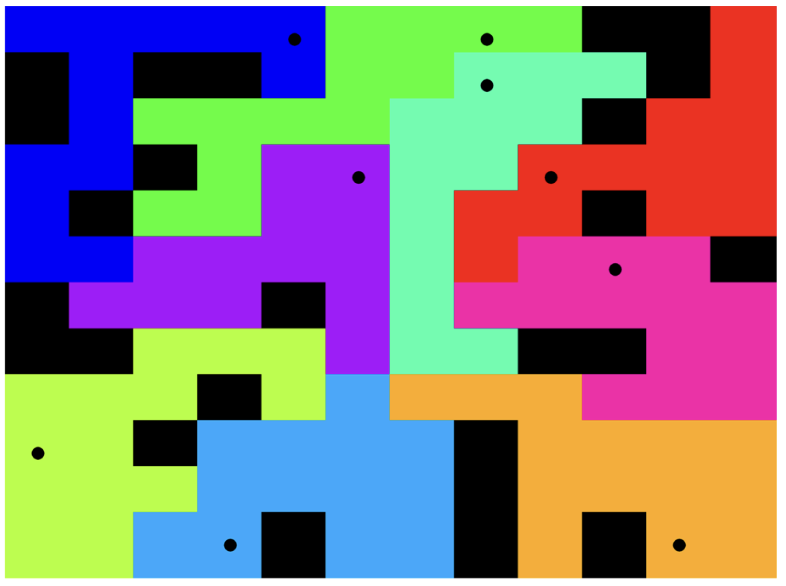
\includegraphics[width=0.45\columnwidth]{fig/darp2.png}
	}
	\\ % Line break for second row
	% Second row of subfigures
	\subfloat[Constructing Minimum Spanning Trees for each one of the robots sets \label{fig:darp3}]{
		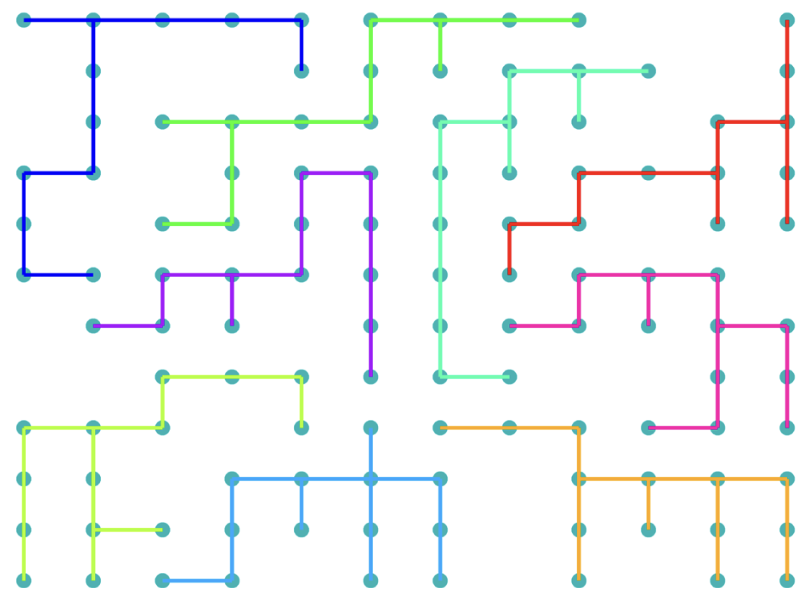
\includegraphics[width=0.45\columnwidth]{fig/darp3.png}
	}
	\hspace{0.1em}
	\subfloat[Final Paths, designed to circumnavigate the MSTs \label{fig:darp4}]{
		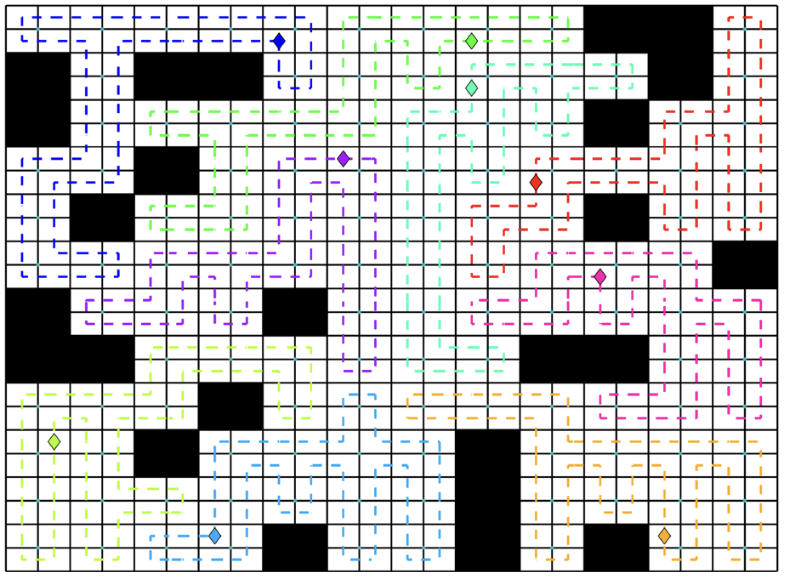
\includegraphics[width=0.45\columnwidth]{fig/darp4.png}
	}
	\caption{DARP+STC Proposed Approach, sample execution with 24x24 grid size, 9 robots and 100 obstacles  \cite{kapoutsisdarp}}
	\label{fig:darp_all}
\end{figure*}

There are $n_r$ robots, with $L_i$ being the robot sets for the $i_{th}$ robot. A selection $L_1, L_2, . . . , L_{n_r}$ poses an optimal solution for the mCPP, iff

\begin{itemize}
	\item $L_i \cap L_j = \emptyset, \quad \forall i, j \in \{1, \ldots, n_r\}, \, i \neq j$
	\item $\bigcup_{i=1}^{n_r} L_i = L$
	\item $\lvert L_1 \rvert \approx \lvert L_2 \rvert \dots \lvert L_{n_r} \rvert$
	\item $L_i \text{ is connected}, \quad \forall i \in \{1, \ldots, n_r\}$
	\item $\chi_i(t_0) \in L_i$
\end{itemize}

The first condition ensures that each cell is assigned exclusively to one robot’s set, enforcing a non-backtracking property in the resulting solution. The second condition specifies that the union of all \(L_i\) sets must cover every unblocked cell within the area, fulfilling the fundamental coverage requirement of completeness. The third condition focuses on maximizing the use of multi-robot dynamics by ensuring that the number of cells \(|L_i|\) in each robot’s set is approximately equal. The fourth condition mandates that each robot’s set \(L_i\) should consist of compact and contiguous cells, forming a cohesive sub-region. This guarantees a fair division and enables seamless navigation within spatially connected areas, preventing robots from spending unnecessary time traveling between disjoint regions. Finally, the fifth condition requires that each robot’s initial position \(\chi_i(t_0)\) is located within its assigned set \(L_i\), ensuring zero preparation time and minimizing energy consumption. Any algorithm capable of constructing the \(L_i\) sets while satisfying these five conditions can be combined with the STC algorithm to produce optimal solutions for the original mCPP problem.

Regarding the existence of such solutions, it has been proven that a fair partition, not restricted to convex regions, always exists for any polygon and any number of partitions. However, the variation of the problem considered here includes an additional condition: the requirement for each partition to contain a specified arbitrary point within the polygon. This added constraint makes the problem dependent on the arrangement of these arbitrary points and means a solution does not always exist. The overall formulation and proposed algorithm address cases where at least one optimal solution is guaranteed to exist.

In the algorithm, until all area division objectives are met, do:
\begin{enumerate}
	\item Assign every \((x, y)\) cell to a robot according to:
	\[
	A(x, y) = \argmin E_i(x, y)
	\]
	Here, $E_i$ is the evaluation matrix for Robot $i$ and  $E_i(x, y)$  is the reachability from $(x, y)$ and the initial position of robot $i$.
	\item For each \(i\)-th robot, where \(i \in \{1, \ldots, N\}\), perform the following steps:
	\begin{enumerate}
		\item Calculate \(k_i\), where $k_i = \lvert L_i \rvert$
		\item Update \(m_i \gets m_i + \eta(k_i - f)\), where $m_i$ is a scalar correction factor for the $i^{th}$ robot, and $f$ denotes the global fair share.
		\item Calculate the connectivity matrix \(C_i\).
		\item Update \(E_i \gets C_i \odot m_i E_i\).
	\end{enumerate}
\end{enumerate}

After the desired area division is achieved, we use Spanning Tree Coverage (STC) algorithm to produce the optimal path for each robot, in order to achieve full coverage of the area of interest.

\section{Drone Swarms}
\rhead{Drone Swarms}
\label{DroneSwarms}

Underwater drones, also known as Unmanned Underwater Vehicles (UUVs), have found significant applications in both civilian and military domains. These versatile vehicles are used in tasks ranging from deep-sea exploration to military operations. A notable area of innovation is \textbf{multi-agent Coverage Path Planning (mCPP)}, which focuses on optimizing the coverage of a defined area using multiple coordinated UUVs. Below are key applications of UUVs leveraging mCPP, supported by real-world examples.

\begin{itemize}
	\item \textbf{Military Applications:}
	\begin{itemize}
		\item \textbf{Mine Countermeasures:}  
		UUVs have been extensively used for mine detection and removal. For instance:
		\begin{itemize}
			\item During the Iraq War, the US Navy deployed UUVs to clear mines around the port of Umm Qasr \cite{RAND}.
			\item The REMUS UUV, a 3-foot-long robot, can clear mines in one square mile within 16 hours, a task that would take human divers over 21 days \cite{REMUS}.
		\end{itemize}
		
		\item \textbf{Data Collection and Reconnaissance:}  
		UUVs collect critical environmental data for military operations. Examples include:
		\begin{itemize}
			\item The Chinese Sea Wing (Haiyi) UUV, found near Indonesia’s Selayar Island in 2020, gathers data such as water temperature, salinity, and oxygen levels to map optimal submarine routes \cite{SeaWing}.
		\end{itemize}
		
		\item \textbf{Submarine Warfare and Surveillance:}  
		Advanced UUVs perform key roles in submarine warfare. For example:
		\begin{itemize}
			\item The Proteus UUV, developed by Huntington Ingalls Industries, utilizes synthetic aperture sonar to identify and neutralize underwater targets. This capability was demonstrated during the 2018 Advanced Naval Technology exercises \cite{Proteus}.
		\end{itemize}
		
		\item \textbf{Multi-Domain Operations:}  
		UUVs with trans-medium capabilities, such as China’s flying submarine drones, extend mCPP applications to both underwater and aerial missions \cite{Harbin2022}.
	\end{itemize}
	
	\item \textbf{Deep-Sea Exploration and Research:}
	\begin{itemize}
		\item \textbf{Mapping and Sample Collection:}  
		UUVs map the ocean floor and collect samples efficiently. Examples include:
		\begin{itemize}
			\item The \textit{Sentry} UUV by the Woods Hole Oceanographic Institution, which can map the seabed at depths of up to 6,000 meters \cite{WHOI}.
		\end{itemize}
		
		\item \textbf{Biodiversity Studies:}  
		UUVs assist in exploring and monitoring underwater ecosystems:
		\begin{itemize}
			\item Researchers have used UUVs to collect samples for studying the microplastic content of ocean floors and assess the health of deep-sea ecosystems \cite{DeepSea2021}.
		\end{itemize}
		
		\item \textbf{Exploration in Extreme Environments:}  
		UUVs are critical for operations in high-pressure environments:
		\begin{itemize}
			\item Bio-inspired soft robots capable of operating in the Mariana Trench have been used for deep-sea exploration and environmental monitoring \cite{Mariana2021}.
		\end{itemize}
	\end{itemize}
	
	\item \textbf{Ecosystem Monitoring and Rehabilitation:}
	\begin{itemize}
		\item \textbf{Water Quality Monitoring:}  
		UUVs are used to monitor and manage water ecosystems. Examples include:
		\begin{itemize}
			\item Duro AUS UUVs deployed in New York City's Randall's Island Park Alliance to monitor wetland health in the East and Harlem Rivers.
		\end{itemize}
		
		\item \textbf{River and Estuary Restoration:}  
		UUVs support environmental rehabilitation initiatives:
		\begin{itemize}
			\item The Bronx River Alliance uses UUVs to monitor and rejuvenate river ecosystems, helping to restore wildlife and improve water quality.
		\end{itemize}
	\end{itemize}
\end{itemize}

\noindent As advancements in robotics, artificial intelligence, and communication technologies continue to advance, the integration of mCPP in UUV operations is expected to expand, enabling transformative applications across military, scientific, and environmental domains.

\noindent This study investigates the application of compositional runtime enforcement in underwater robotic swarms, evaluating its performance in comparison to the conventional monolithic approach. The research focuses on integrating runtime enforcement into a Multi-Robot Coverage Path Planning (MRCPP) algorithm tailored for mapping underwater vegetation in seagrass beds. By analyzing both methods, the study seeks to determine their influence on the algorithm's efficiency, scalability, and flexibility in dynamic underwater conditions.

\begin{figure}[htb]
	\centering
	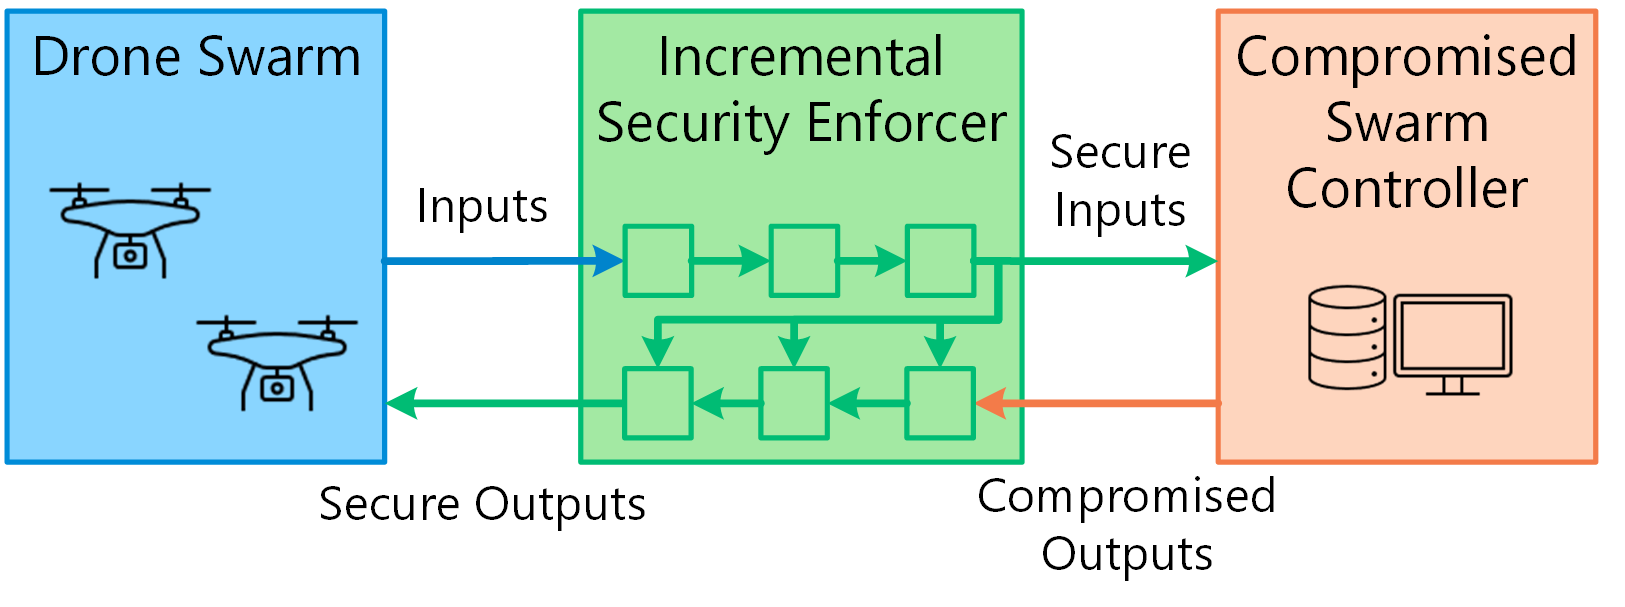
\includegraphics[width=0.94\linewidth]{fig/drone-system2.png}
	\caption{System diagram of incremental enforcement for a drone swarm.}
	\label{fig:drone-system}
\end{figure} 


\section{Attack On Drones}
\rhead{Attack On Drones}
\label{AttackOnDrones}

While underwater drones offer significant benefits in exploration, research, and military applications, they are not immune to threats from malicious actors. Recent work by Yaacoub et al. in \cite{yaacoub2020security} surveys a range of attacks on robotic systems. Underwater drones are particularly vulnerable to interference and manipulation due to their reliance on acoustic communication and complex navigation systems. For instance, acoustic jamming and spoofing attacks can disrupt communication and navigation, leading to miscoordination or loss of control \cite{westerlund2019drone}. Additionally, acoustic or magnetic interference can trigger emergency behaviors, such as premature surfacing or drifting \cite{Abunada2020}, and prevent the relay of vital status and control signals \cite{Valianti2021}. This disruption in communication between drones and the central controller can lead to unsafe outcomes, including collisions, mission failure, or environmental damage.

Hardware vulnerabilities, such as tampered communication modules or sensor systems \cite{belous2020hardware}, provide opportunities for attackers to inject, intercept, or alter control commands. Such attacks can force underwater drones to violate operational boundaries, collide with obstacles, or fail to execute their intended tasks.

In this work, we consider five potential attacks on an underwater drone swarm's coordinated operation:
\begin{itemize}
	\item[A1] \emph{Boundary Breach} \textit{(Injection and Alteration)}: where the attacker manipulates control signals to force drone(s) to leave their designated operational area, potentially breaching restricted zones or damaging sensitive ecosystems.
	\item[A2] \emph{Overwhelm Inputs} \textit{(Injection and Alteration)}: an attack where drone(s) are overloaded with conflicting or erroneous control signals, leading to erratic behavior or mission disruption.
	\item[A3] \emph{Block Control Signals} \textit{(Jamming)}: any attack that disrupts acoustic or RF communication, preventing updated control signals from reaching one or more drone(s) in the swarm.
	\item[A4] \emph{Drain Power} \textit{(Injection and Alteration)}: where the attacker commands drones to perform energy-intensive tasks, such as high-speed maneuvers or prolonged thruster usage, depleting their batteries prematurely.
	\item[A5] \emph{Pressure Limit Violation}  \textit{(Injection and Alteration)}: an attack where an adversary disrupts the simultaneous execution of pressure limit monitoring and ascent actions. This could cause drones to remain at unsafe depths, risking structural failure due to high pressure, or to ascend improperly, compromising mission integrity or safety.
\end{itemize}

We categorize these attacks into common types: \textit{jamming} and \textit{injection and alteration}. \textit{Injection and alteration} attacks involve the addition or manipulation of control packets, while \textit{jamming} attacks remove or block communication packets. To mitigate these threats, we develop robust policies enforced through a compositional runtime enforcement framework tailored to underwater drone operations.


\section{Mitigation with Enforcement}
\rhead{Mitigation with Enforcement}
\label{MitigationwithEnforcement}

This work defines a series of security policies to mitigate attacks on underwater drones. These policies are enforced through a runtime enforcement framework to ensure safe and secure operation, even in the presence of malicious interference. The inputs and outputs for each drone are defined as follows:

\begin{itemize}
	\item Inputs ($I$): $\lbrace \mathsf{left\_boundary}, \mathsf{right\_boundary}, \mathsf{down\_boundary}, \mathsf{up\_boundary}, \mathsf{rpm\_limit}, \mathsf{pressure\_limit} \rbrace$ (signals from the plant to the controller).
	\item Outputs ($O$): $\lbrace \mathsf{up}, \mathsf{down}, \mathsf{right}, \mathsf{left}, \mathsf{rpm\_up}, \mathsf{rpm\_down}, \mathsf{ascent} \rbrace$ (control actions sent from the controller to the plant).
\end{itemize}

The following policies correspond to the identified attacks and define mitigation strategies:

\begin{itemize}
	\item \textbf{Policy $\varphi_1$: Boundary Breach (Prevents A1)}  
	This policy ensures that drones do not violate predefined operational boundaries. It enforces the following:
	\begin{itemize}
		\item $\mathsf{left\_boundary}$ and $\mathsf{left}$ cannot occur simultaneously.
		\item $\mathsf{right\_boundary}$ and $\mathsf{right}$ cannot occur simultaneously.
		\item $\mathsf{down\_boundary}$ and $\mathsf{down}$ cannot occur simultaneously.
		\item $\mathsf{up\_boundary}$ and $\mathsf{up}$ cannot occur simultaneously.
	\end{itemize}
	
	\item \textbf{Policy $\varphi_2$: Conflicting Signals (Prevents A2)}  
	This policy ensures no simultaneous conflicting control signals are sent to the drone. It enforces the following:
	\begin{itemize}
		\item $\mathsf{left}$ and $\mathsf{right}$ cannot occur simultaneously.
		\item $\mathsf{up}$ and $\mathsf{down}$ cannot occur simultaneously.
		\item $\mathsf{rpm\_up}$ and $\mathsf{rpm\_down}$ cannot occur simultaneously.
	\end{itemize}
	
	\item \textbf{Policy $\varphi_3$: Block Control Signals (Prevents A3)}  
	This policy mandates that drones ascend to the surface when control signals are not received for a specific time threshold (5 seconds). It enforces:
	\begin{itemize}
		\item If no input or output signals are received, and the timer exceeds 5 seconds, then the drone ascends to the surface.
	\end{itemize}
	
	\item \textbf{Policy $\varphi_4$: Drain Batteries (Prevents A4)}  
	This policy ensures that the $\mathsf{rpm\_up}$ signal does not occur simultaneously with $\mathsf{rpm\_limit}$. It enforces:
	\begin{itemize}
		\item $\mathsf{rpm\_up}$ and $\mathsf{rpm\_limit}$ cannot occur simultaneously.
	\end{itemize}
	
	\item \textbf{Policy $\varphi_5$: Pressure Limit and Ascent Coordination (Prevents A5)}  
	This policy ensures that $\mathsf{pressure\_limit}$ and $\mathsf{ascent}$ occur simultaneously. It enforces:
	\begin{itemize}
		\item $\mathsf{pressure\_limit}$ and $\mathsf{ascent}$ must occur simultaneously.
	\end{itemize}
\end{itemize}

These policies collectively address key threats to underwater drones and ensure secure and reliable operations in dynamic and potentially adversarial environments.

\subsubsection{Policy $\varphi_{1}$ mitigating attack A1, \emph{Boundary Breach}}

The \emph{Boundary Breach} attack occurs when a drone is instructed to violate predefined airspace boundaries or the separation limits between drones. To mitigate this, Policy $\varphi_1$ ensures that the drone operates within its allowed 2D workspace while moving in four primary directions: left, right, up, and down. The drone is prevented from breaching boundaries or failing to move when expected. Specifically, for the \textbf{left} direction:

\begin{itemize}
	\item If the drone attempts to move left while already at the left boundary (\texttt{left\_boundary} $\land$ \texttt{left}), it is considered a violation, and the drone's left movement is disabled (\texttt{left := 0}).
	\item If the drone fails to move left when not at the left boundary ($\neg$ \texttt{left\_boundary} $\land$ $\neg$ \texttt{left}), the policy forces left movement (\texttt{left := 1}).
\end{itemize}

The same logic applies for the other directions (\textbf{right}, \textbf{up}, and \textbf{down}) with their respective boundary conditions (\texttt{right\_boundary}, \texttt{up\_boundary}, \texttt{down\_boundary}). This policy ensures that the drone adheres to boundary constraints, preventing it from breaching airspace limits or failing to navigate appropriately within the defined 2D area.


\begin{figure}[H]
	\centering
	\begin{tikzpicture}[->,shorten >=1pt,auto,node distance=4cm,semithick]
		
		% Styles for the states
		\tikzstyle{state}=[circle,thick,draw=green!75,fill=green!20,minimum size=8mm]
		\tikzstyle{accepting state}=[state, double]
		\tikzstyle{violation state}=[circle,thick,draw=red!75,fill=red!20,minimum size=8mm]
		
		% Nodes for the DFA
		\node[accepting state,initial] (l0) {$l_0$};
		\node[violation state] (lv) [right=6cm of l0] {$l_v$};
		
		% Transitions from l0 to lv with adjusted label placement
		\path
		(l0) edge[bend left=50] node[above] {\scriptsize $\neg (\text{left} \oplus \text{left\_boundary})$} (lv)
		(l0) edge[bend left=20] node[above] {\scriptsize $\neg (\text{right} \oplus \text{right\_boundary})$} (lv)
		(l0) edge[bend right=20] node[below] {\scriptsize $\neg (\text{up} \oplus \text{up\_boundary})$} (lv)
		(l0) edge[bend right=50] node[below] {\scriptsize $\neg (\text{down} \oplus \text{down\_boundary})$} (lv)
		
		% Self-loop on violation state
		(lv) edge[loop right] node {$\Sigma$} (lv);
		
	\end{tikzpicture}
	\caption{Automaton for policy $\varphi_{1}$ which prevents a drone from breaching its boundary}
	\label{fig:p1}
\end{figure}

\subsubsection{Policy $\varphi_{2}$ mitigating attack A2, \emph{Overwhelm Inputs}}

In attack A2, \emph{Overwhelm Inputs}, the attacker sends conflicting control signals to the drone. Policy $\varphi_{2}$ is designed such that simultaneously present conflicting controls cause violation. The synthesised enforcer will therefore suppress one of these conflicting signals to ensure the drone is not overwhelmed.

\begin{figure}[H]
	\centering
	\begin{tikzpicture}[->,shorten >=1pt,auto,node distance=4cm,semithick]
		% Styles for the states
		\tikzstyle{state}=[circle,thick,draw=green!75,fill=green!20,minimum size=8mm]
		\tikzstyle{accepting state}=[state, double]
		\tikzstyle{violation state}=[circle,thick,draw=red!75,fill=red!20,minimum size=8mm]
		
		% Nodes for the DFA
		\node[accepting state,initial] (l0) {$l_0$};
		\node[violation state] (lv) [right=6cm of l0] {$l_v$};
		
		% Transitions from l0 to lv with adjusted label placement
		\path
		(l0) edge[bend left=20] node[above] {\scriptsize $left \land right$} (lv)
		(l0) edge[bend left=0] node[below] {\scriptsize $up \land down$} (lv)
		(l0) edge[bend right=20] node[below] {\scriptsize $rpm\_up \land rpm\_down$} (lv)
		
		% Self-loop on violation state
		(lv) edge[loop right] node {$\Sigma$} (lv);
	\end{tikzpicture}
	\caption{Automaton for policy $\varphi_{2}$ which prevents overwhelming of the inputs}
	\label{fig:p2}
\end{figure}


\subsubsection{Policy $\varphi_{3}$ mitigating attack A3, \emph{Block Control Signals}}

The attack A3, \emph{ Block Control Signals}, which jams signals prevents the drone from getting updated controls. This could result in it continuing to climb or move in undesirable ways. The policy detects if no control signals are sent in any 5-second period. The drone is then brought to the surface using the \texttt{ascent} signal.


\begin{figure}[H]
	\centering
	\begin{tikzpicture}[->,shorten >=1pt,auto,node distance=4cm,semithick]
		
		% Styles for the states
		\tikzstyle{state}=[circle,thick,draw=green!75,fill=green!20,minimum size=8mm]
		\tikzstyle{accepting state}=[state, double]
		\tikzstyle{violation state}=[circle,thick,draw=red!75,fill=red!20,minimum size=8mm]
		
		% Nodes for the DFA
		\node[accepting state,initial] (l0) {$l_0$};
		\node[accepting state] (l1) [right=6cm of l0] {$l_1$};
		\node[violation state] (lv) [right=6cm of l1] {$l_v$};
		
		% Transitions
		\path
		% Transition from l0 to l1
		(l0) edge[bend left=15] node[above] {\scriptsize \parbox{2cm}{$\Sigma$ \\ ($t := 0$)}} (l1)
		
		% Transition from l1 to l0
		(l1) edge[bend left=15] node[below] {\scriptsize \parbox{2.5cm}{$ascent \land$ $(t > 5s)$}} (l0)
		
		% Self-loop on l1
		(l1) edge[loop above] node[above] {\scriptsize \parbox{2cm}{$\Sigma$ \\ ($t := 0$)}} (l1)
		
		% Transition from l1 to lv
		(l1) edge[bend left=15] node[above] {\scriptsize \parbox{2.5cm}{$\neg ascent \land$ $(t > 5s)$}} (lv)
		
		% Self-loop on lv
		(lv) edge[loop right] node[above] {\scriptsize $\Sigma$} (lv);
		
	\end{tikzpicture}
	\caption{Automaton for policy $\varphi_{3}$ which ensures safe transitions based on timeout and ascent conditions.}
	\label{fig:p3}
\end{figure}


\subsubsection{Policy $\varphi_{4}$ mitigating attack A4, \emph{Drain Batteries}}

Attack A4, \emph{Drain Batteries}, involves injection or alteration of signals to increase the drone's RPM beyond the efficiency threshold, which is crucial for maintaining optimal flight endurance during the QR display. Although higher RPM allows faster movement, it significantly reduces efficiency, causing the battery to deplete more rapidly. To mitigate this, an RPM limit is enforced. Policy $\varphi_{4}$ is a simple policy which prevents $rpm\_up$ signal when $rpm\_limit$ is active.

\begin{figure}[H]
	\centering
	\begin{tikzpicture}[->,shorten >=1pt,auto,node distance=5cm,semithick]
		
		% Styles for the states
		\tikzstyle{state}=[circle,thick,draw=green!75,fill=green!20,minimum size=8mm]
		\tikzstyle{accepting state}=[state, double]
		\tikzstyle{violation state}=[circle,thick,draw=red!75,fill=red!20,minimum size=8mm]
		
		% Nodes for the DFA
		\node[accepting state,initial] (l0) {$l_0$};
		\node[violation state] (lv) [right=6cm of l0] {$l_v$};
		
		% Transitions
		\path
		% Self-loop on l0
		(l0) edge[loop above] node[above] {\scriptsize $\Sigma$ / ($rpm\_up \land rpm\_limit$)} (l0)
		
		% Transition from l0 to lv
		(l0) edge[bend left=0] node[above] {\scriptsize $rpm\_up \land rpm\_limit$} (lv)
		
		% Self-loop on lv
		(lv) edge[loop right] node[above] {\scriptsize $\Sigma$} (lv);
		
	\end{tikzpicture}
	\caption{Automaton for policy $\varphi_{4}$ which ensures safe RPM limits to prevent battery drain.}
	\label{fig:p4}
\end{figure}

\subsubsection{Policy $\varphi_{5}$ mitigating attack A5, \emph{Pressure Limit Violation}}

Attack A5, \emph{Pressure Limit Violation}, occurs when an adversary prevents the drone from initiating ascent even when the pressure limit is reached. This attack exploits the safety mechanism designed to protect the drone from operating at unsafe depths, potentially leading to structural damage or mission failure. To mitigate this, Policy $\varphi_{5}$ ensures that the drone immediately triggers the \texttt{ascent} signal whenever the \texttt{pressure\_limit} condition is met, preventing prolonged exposure to high-pressure environments. This simple policy blocks operations that ignore the \texttt{pressure\_limit} condition, ensuring safe and reliable behavior.

\begin{figure}[H]
	\centering
	\begin{tikzpicture}[->,shorten >=1pt,auto,node distance=5cm,semithick]
		
		% Styles for the states
		\tikzstyle{state}=[circle,thick,draw=green!75,fill=green!20,minimum size=8mm]
		\tikzstyle{accepting state}=[state, double]
		\tikzstyle{violation state}=[circle,thick,draw=red!75,fill=red!20,minimum size=8mm]
		
		% Nodes for the DFA
		\node[accepting state,initial] (l0) {$l_0$};
		\node[violation state] (lv) [right=6cm of l0] {$l_v$};
		
		% Transitions
		\path
		% Self-loop on l0
		(l0) edge[loop above] node[above] {\scriptsize $\Sigma$ \textbackslash\ ($pressure\_limit \land \neg ascent$)} (l0)
		
		% Transition from l0 to lv
		(l0) edge[bend left=0] node[above] {\scriptsize $pressure\_limit \land \neg ascent$} (lv)
		
		% Self-loop on lv
		(lv) edge[loop right] node[above] {\scriptsize $\Sigma$} (lv);
		
	\end{tikzpicture}
	\caption{Automaton for policy $\varphi_{5}$ which ensures ascent is triggered when the pressure limit is reached.}
	\label{fig:p5}
\end{figure}










